%%%%%%%%%%%%%%%%%%%%%%%%%%%%%%%%%%%%%%%%%%%%%%%%%%%%%%%%%%%%%%%%%%%%%%%%%%%%%%%%
%%%%%%%%%%%%%%%%%%%%%%%%%%%%%%%%%%%%%%%%%%%%%%%%%%%%%%%%%%%%%%%%%%%%%%%%%%%%%%%%
\section{\textcolor{red}{Percebendo frases musicais}}
\index{Musicalidade!Frase musical}

quando a musica inclue letra es mas fácil distinguir donde inicia y termina la frase.


\subsection{Separando frases analiticamente}

Contando e medindo a frase musical

\cite[pp. 148,150]{medteoria}

\cite[pp. 336]{medteoria}

o cumprimento de frase mais comum é
de 4 compassos \cite[pp. 624]{latham2008diccionario} \cite[pp. 335]{medteoria} \cite[pp. 34]{bennett1993elementos},
tabem é usado cumprimentos de 8 compassos \cite[pp. 335]{medteoria} \cite[pp. 34]{bennett1993elementos}
e 2 compassos \cite[pp. 34]{bennett1993elementos}.
São menos comuns frases de 3,5, ou 7 compassos \cite[pp. 34]{bennett1993elementos}.

Ver Figura \ref{fig:contagemtemposfrase}.
\begin{figure}
    \centering
    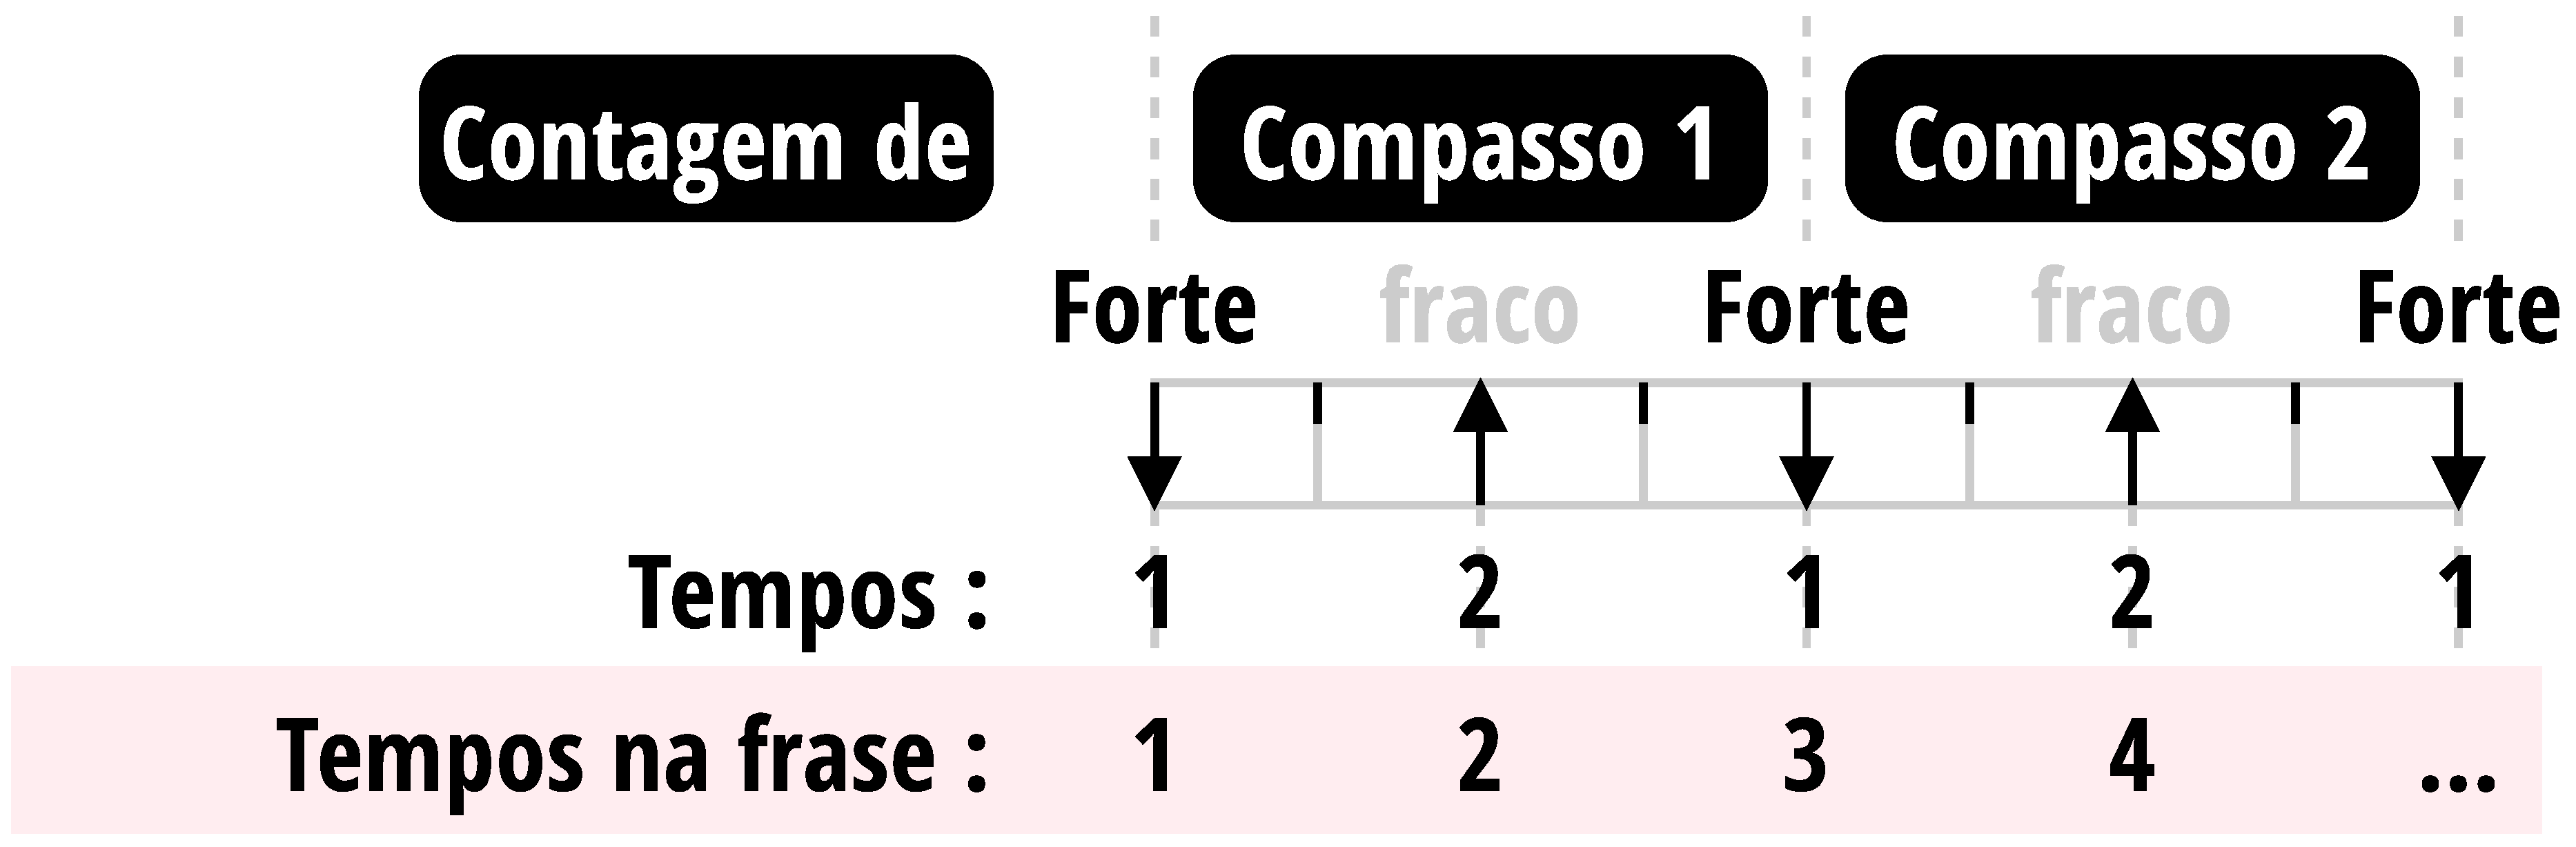
\includegraphics[width=\textwidth]{chapters/cap-musicalidade/contagemtemposfrase.eps}
    \caption{Contando a frase musical.}
    \label{fig:contagemtemposfrase}
\end{figure}



\subsection{Separando frases intuitivamente}


\begin{example}
Usando unicamente a silaba ``la'', crie um discurso; por exemplo:
\begin{citando}%%
Lálala la lalá la lalalá!\\
lá lalá la lálala,\\
la lalalá lála?\\
lá lalá la lalalá.\\
\end{citando}%%
Logo proceda a ler acentuando, pausando e
executando signos de interrogação e admiração;
perceba que o conteúdo das palavras não existe, 
porem pela expressividade na leitura,
é possível extrair dos sonidos produzidos,
onde existem acentos, pausas, e signos de admiração ou interrogação.

Ao escutar uma música, como por exemplo ``Brasileirinho''  de Valdir Azevedo, 
e tentar extrair caraterísticas, acontecerá o mesmo que com o discurso com ``la'', e observaremos que:
\begin{itemize}
\item Teremos uma noção de acentos na melodia, e poderemos intuir fazendo um levantamento estatístico,
em que tempo está localizado o tempo forte; o analises terá que ser probabilístico,
pois existe na música a acentuação de tempos fracos (\hyperref[fig:contratempo]{\textbf{contratempos}}); 
pelo que se alguns tempos não cumprem com nossa predição podemos catalogar eles como contratempos.
\item Podemos perceber as pausas e deduzir que existe um final de \hyperref[fig:Frase]{\textbf{frase}} musical,
ate intuir que pode ter uma \hyperref[fig:Cesura]{\textbf{cesura}}.
\item Também podemos perceber diferentes formas de finalizar uma frase, 
que na linguagem falada associaríamos com o uso ou não de signos de admiração e exclamação;
no âmbito da música, temos algo similar com o uso das \hyperref[fig:Cadencia]{\textbf{cadencias}}.
Assim, cada tipo de cadência nos dará uma ideia diferente da função que cumpre a frase no discurso da peça musical.
\end{itemize}
\end{example}

\subsection{Percebendo o tipo de final da frase}

Porque é importante reconhecer as frases com final conclusivo e suspensivo,
\begin{itemize}
\item Si tentamos dançar no tempo forte, conhecer a existência de ambos tipos de final de frase, 
no ajuda a ter certeza que estamos indo bem com o tempo, e que não somos nos que erramos achando o tempo forte,
e sim, que existe mais de um tipo de final de frase, e que este foi diferente, foi suspensivo.
E não nos deixaremos enganar por finais suspensivos sincopados (que parecem conclusivos),
e estaremos mais seguros de nossa dança.
\item Uma vez temos ciência da existência de ambos tipos de final, 
podemos usar suas particularidades. Por exemplo,
uma frase com final conclusivo indica o fim, literal, de uma ideia musical, 
pelo que si desejamos ter coerência com a música, 
nosso movimento e parada deve demostrar a mesma resolução,
e dar a ideia de que o relato de nossa dança acabou de expressar uma ideia completa;
para isto podemos fazer um movimento explosivo com pausa abrupta, 
ou agregar uma postura final, ou tao simples como um abraço elegante com ponto final.
Por outro lado, se o final de frase musical é suspensivo, 
a ideia transmitida tem uma sensação de pergunta,
ou de uma resposta meditativa que se apaga aos poucos e pede uma reflexão ao ouvinte,
em outras palavras um assunto não completamente  concluído.
Nesse sentido, se nosso objetivo é ter uma coerência com a música,
o relato que expressa nossa dança deve dar essa sensação de uma ideia que se apaga aos poucos,
ou de pergunta; por exemplo, isto se consegue dando um passo final em tempo forte,
seguido de movimentos corporais no lugar ate a ultima nota musical.
\end{itemize}

Exemplo de final conclusivo e suspensivo na Figura \ref{fig:conclusivo-suspensivo1}. 

\begin{figure}[H]
\centering
\begin{abc}[name=abc-conclusivo-suspensivo1]
X: 1 % start of header
K: C stafflines=1 % scale: C major
M: 2/4 %meter - compasso
L:1/8
Q:1/4=80
V:1 clef=perc stem=down %name="Pauta com clave de fá"   sname="Pauta com clave de fá"
[V:1] |:B3/2 B/2 B1 B1| B/2  B2 z/2  z1 | B3/2 B/2 B1 B1| B2 z2:|
w:      TA!  ti-ta-ta   TI!-ta             TA!  ti-ta-ta  TA!
\end{abc}
\caption{Frase de 8 tempos.}
\label{fig:conclusivo-suspensivo1}
\end{figure}



\subsubsection{\textcolor{red}{percebendo frases com final conclusivo}}
% Breaks (frases com final conclusivo):
% Moreira Da Silva - Idade Não é Documento - https://www.youtube.com/watch?v=-mwwkz3TwxU
% JOGANDO COM O CAPETA MOREIRA DA SILVA - https://www.youtube.com/watch?v=MYngGP43lkY
% ??? Moreira Da Silva - Na Subida Do Morro - https://www.youtube.com/watch?v=fD8Hh4CFPkk

\subsubsection{\textcolor{red}{percebendo frases com final suspensivo}}

% Breaks (Voz: frases final conclusivo + suspensivo + contratempo)
% https://www.youtube.com/watch?v=ujEDJhBx2W0
% Breaks (voz: frases final conclusivo + suspensivo):
% https://www.youtube.com/watch?v=YC9nVbVrUHU

\subsubsection{\textcolor{red}{percebendo frases com final suspensivo a contratempo e sincopado}}
% Breaks (voz: frases final suspensivo + sincopado):
% Eu Sou A Marrom - https://www.youtube.com/watch?v=QMUkDngZmjo



